% Introduction of the discussion


% May move this subsection to the discussion.
\subsection{Age-related conflict : who are the winners ?}

So far, the labor share has been declining due to the baby-boomers generation in both countries. First, when they were young because they shaped the public policy and so the labor market institutions in their favor. The firms answered to that by substituting labor to capital. Second, when they were old because they have considerably increased the available capital in the economy through savings allowing the firms to substitute even more. However, the labor income share is a gross indicator of inequalities. A more appropriate indicator may be the income ratio between young and old after redistribution. 

From equation \eqref{eq:after_tax_income_ratio}, I have that the after-tax young-to-old income ratio is equal to the young political weight (i.e. $Y_t^y/Y_t^o = \eta_t$). While the before-tax young-to-old income ratio corresponds to the labor-to-capital ratio (i.e. $\Theta_t = \frac{w_tL_t}{r_tK_t}$). Figure \ref{fig:raw_vs_net_inc_ratio} displays these income ratios in deviation from the 1970 steady-state.
\begin{figure}[tb]
	\centering
		\caption{Deviation from 1970's value of the labor-to-capital income ratio and the young-to-old income ratio} \label{fig:raw_vs_net_inc_ratio}
	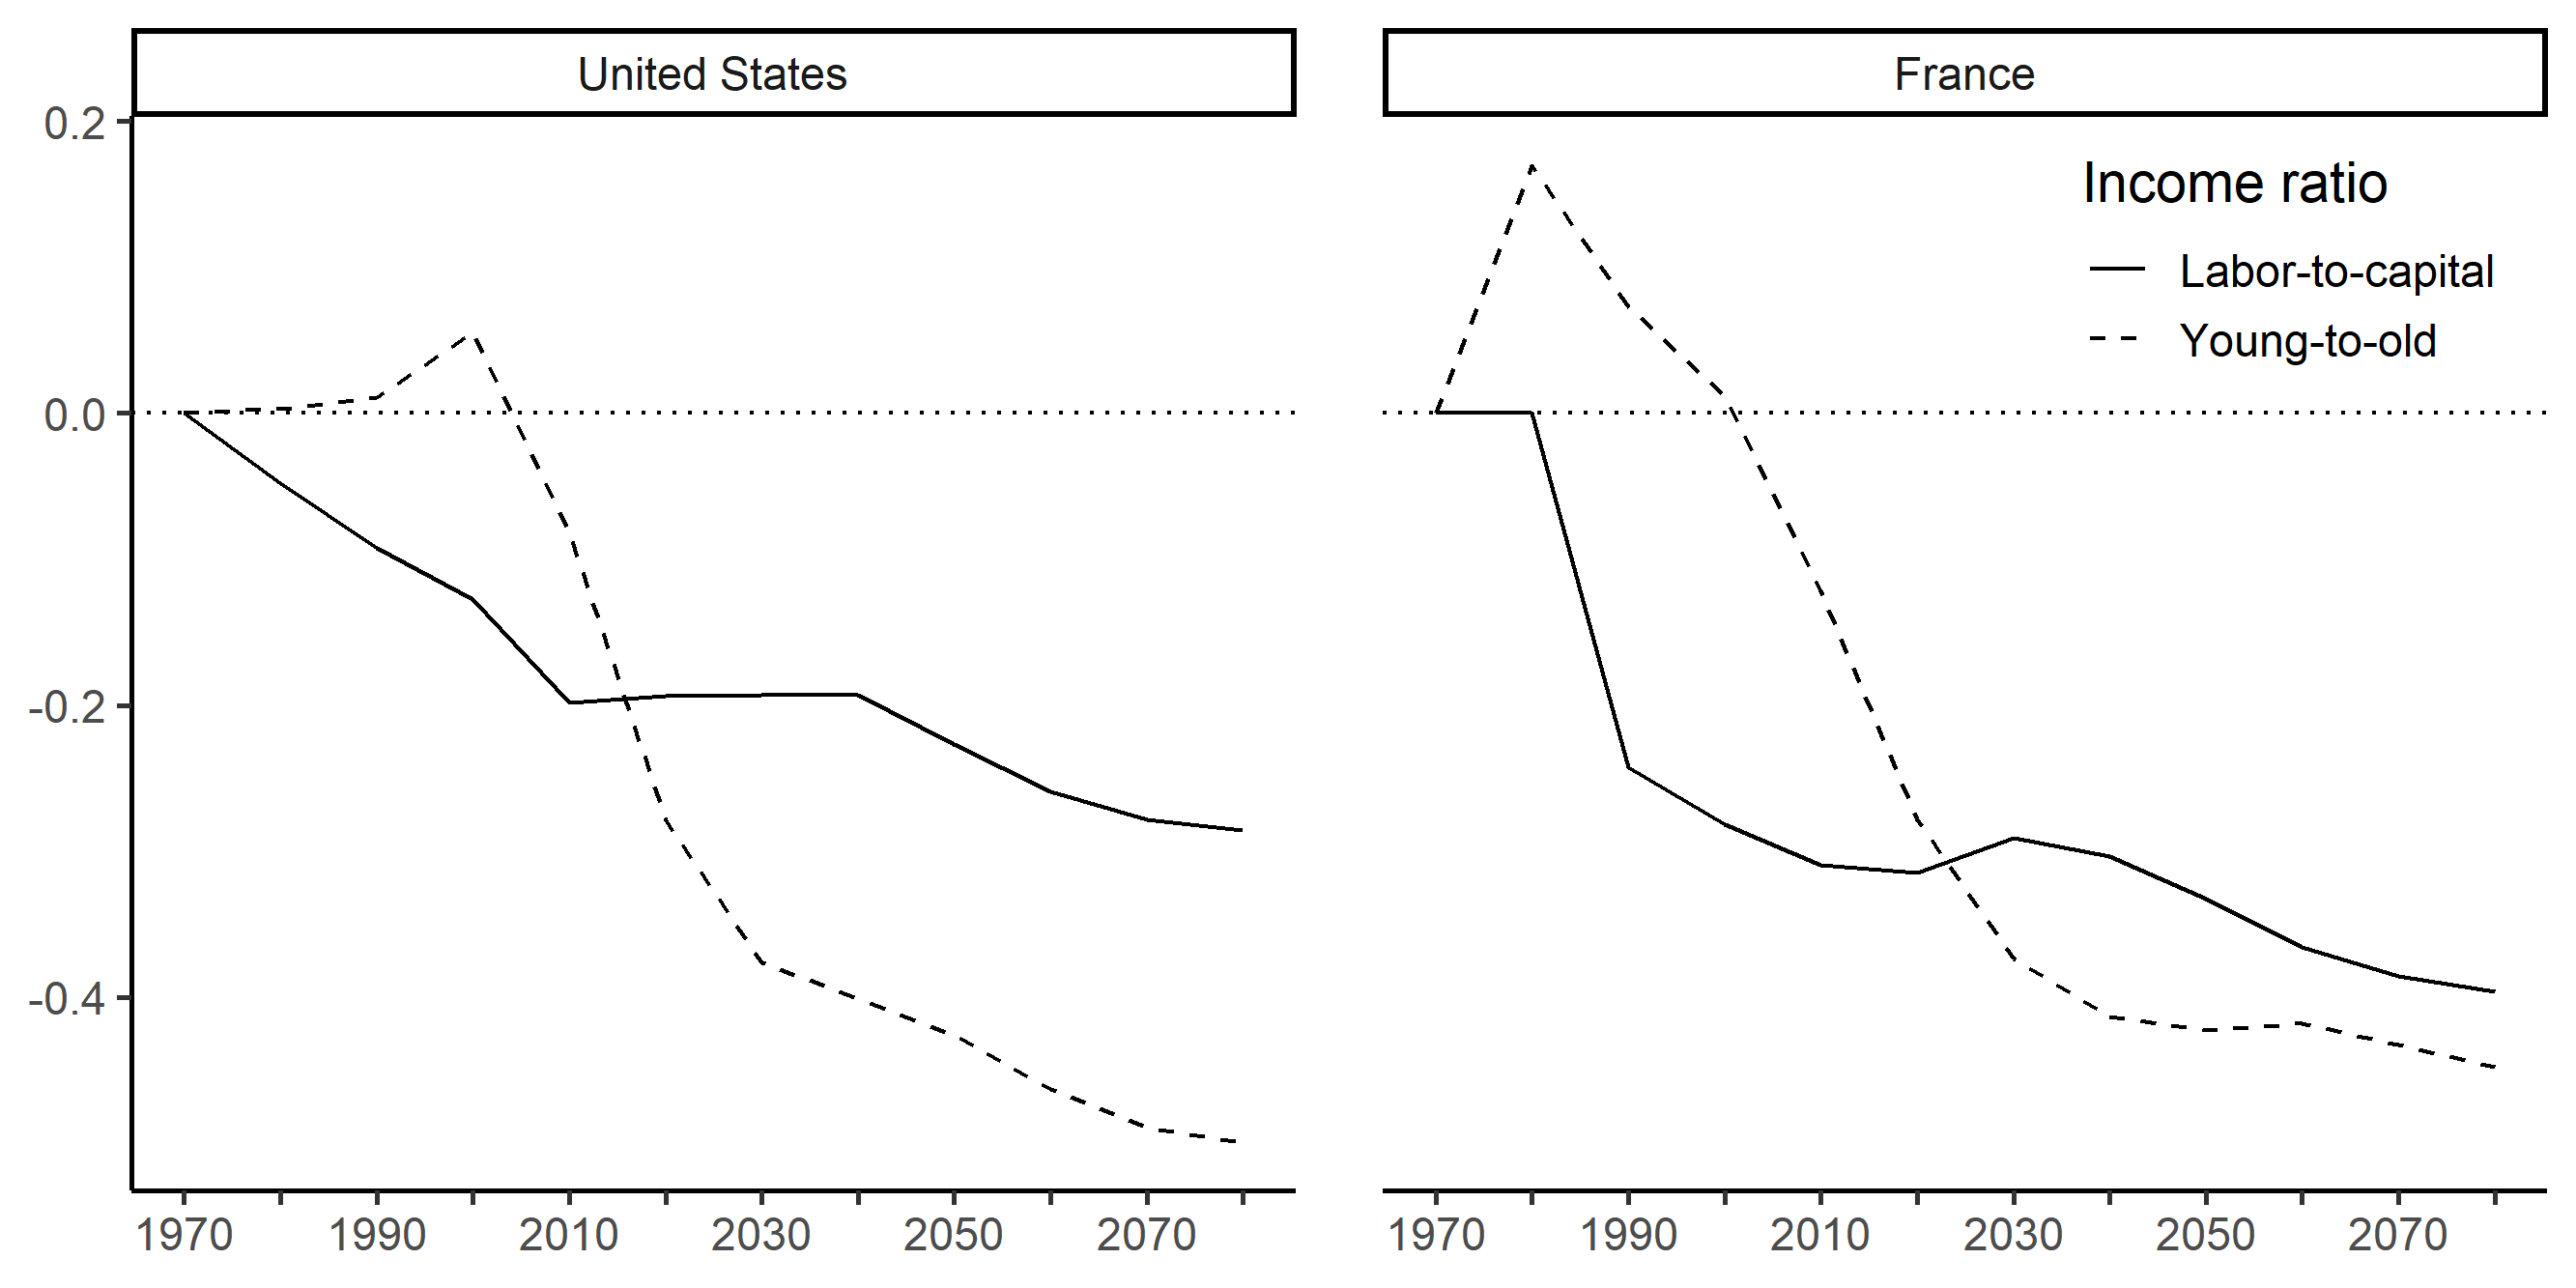
\includegraphics[width=1\linewidth]{../result/redistribution/dev_incratio_raw_vs_net.png}
	\vspace{-6ex}
	\justify\singlespacing\footnotesize The solid curve corresponds to the before-tax young-to-old income $\Theta_t$ ratio also named the labor-to-capital income ratio $\frac{w_tL_t}{r_tK_t}$ and the dashed curve is the after-tax young-to-old income ratio $Y_t^y/Y_t^o$ which is equal to the youth political power $\eta_t$. Deviation is expressed in percentage.
	% and the dotted line is the after-tax young-to-old income ratio with government health spending included in old households income $Y_t^y/(Y_t^o+h_tN_t^o$).
\end{figure}
While the labor share and so the labor-to-capital ratio (i.e. before-tax young-to-old income ratio) sharply decline between 1970 and 2000, the after-tax young-to-old income ratio lies over its 1970's level during the same period. Even if I include the government health spending as part of the old households income, the young-to-old income ratio remains over its initial level until 2000.\footnote{In terms of deviation, the curve is combined with the dashed one.} This model prediction holds for both countries. The baby-boomers gross income share (i.e. labor income share) has declined due to the mechanisms previously mentioned when they were young. However, they also have spurred political parties to implement redistributive public policies.\footnote{This is the result of the probabilistic voting specification. The opportunist behavior of political parties lead them to favor this generation in order to maximize their probability to win the election.} This redistribution is characterized, in terms of the model, through a raise of the tax rate and an increase of the unemployment spending share within the government revenue.\footnote{Notice that the increase of the unemployment spending share is driven and accentuated by the raising unemployment due to factor substitution.} Thus, they have been able to seize part of their elders income through redistribution. Even though baby-boomers appeared as income losers over this period because the labor share was falling, they are actually the winners once net income is considered.

Another way to determine the winners of the age-related conflict within the public policy is to look how the GDP is allocated in the economy. Figure \ref{fig:redis_step3_stacked} displays the income allocation after redistribution.
\begin{figure}[tb]
	\centering
	\caption{After-tax income share allocation} \label{fig:redis_step3_stacked}
	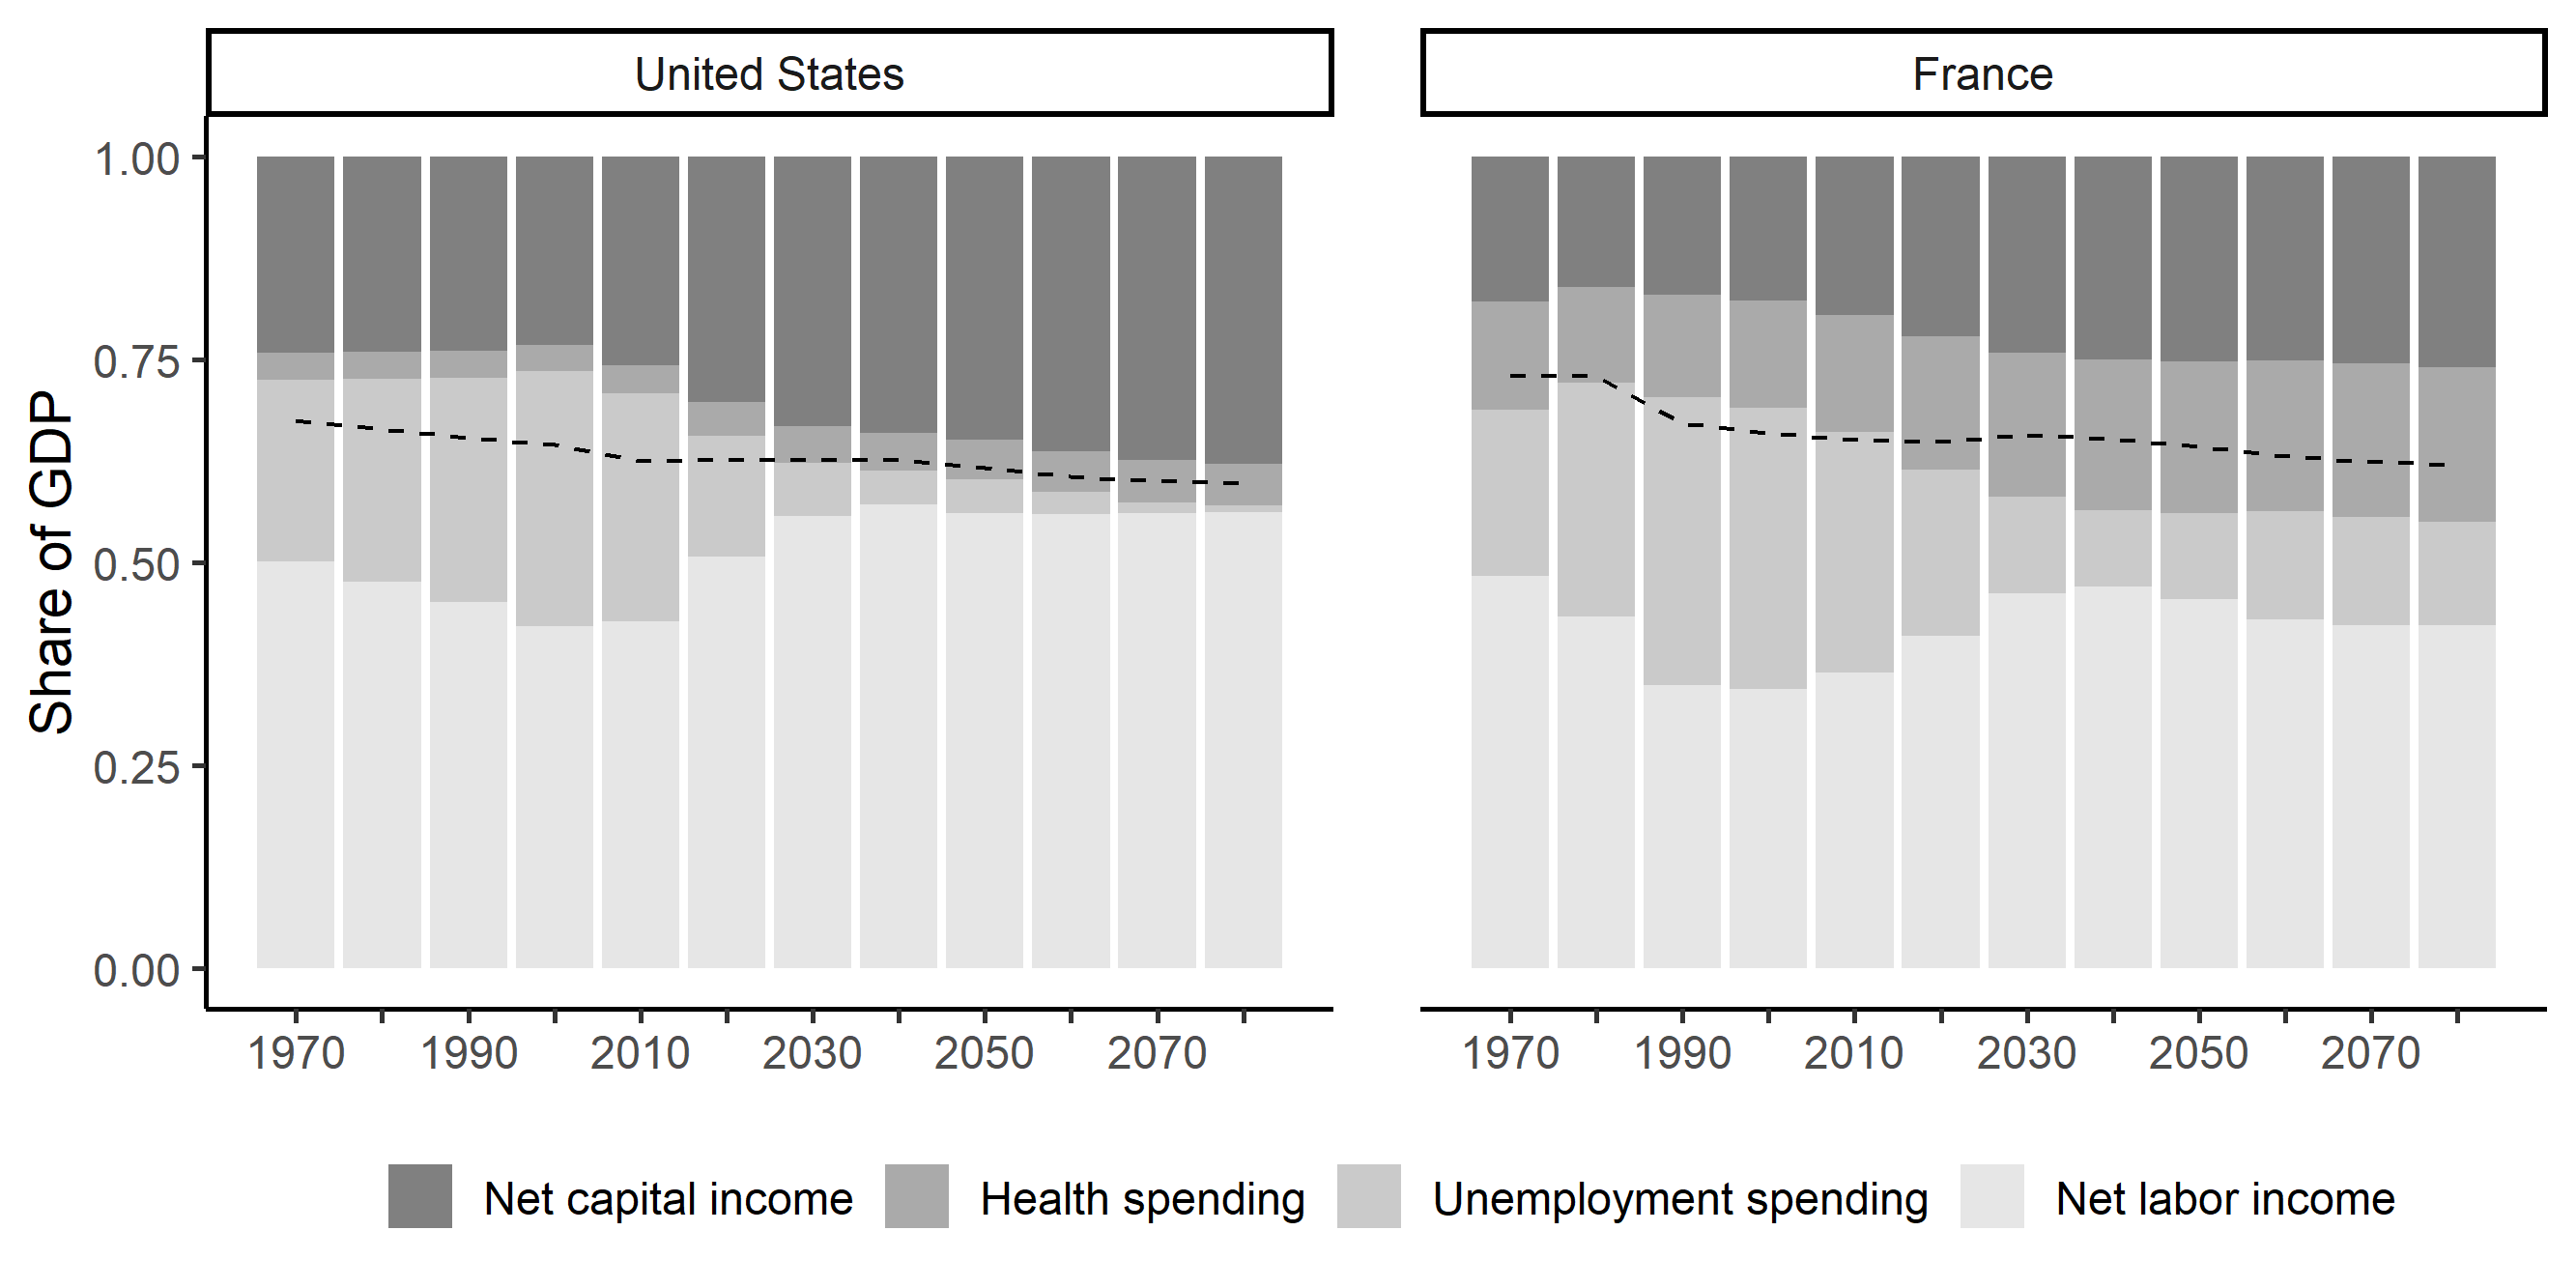
\includegraphics[width=1\linewidth]{../result/redistribution/redis_step3_stacked.png}
\end{figure}
The dashed curve corresponds to the labor share, so the before-tax young income share. As long as this curve lies in the area of the government unemployment spending share, it means that old agents fund unemployment spending through their taxes. On the contrary, when the dashed curve lies in the area of the government health spending share, the young agents fund government health spending for their elders. The US share of GDP which is allocated to health spending is quite small compared to the French one. This is directly related to the preference parameter for government health spending $\beta$.\footnote{$\beta_{\text{FR}} = 0.739$ and $\beta_{\text{US}} = 0.138$.} The US young generations are the winners of the age-related conflict from 1970 to 2020 which corresponds to the active period of the baby-boomers. Once the US population ages and therefore the baby-boomers, old households dominates the public policy conflict. However, the size of the government revenue declines due to the fact that the United-States converges to full employment in the long run. For France, the baby-boomers also dominate the public policy conflict between 1990 and 2010 when they are active. Once they retire, so over the period 2010-2040, they are still the winners of this conflict and their children fund government health spending. Notice that the size of the welfare state corresponds to the sum of the unemployment benefits share in GDP and the health spending share in GDP.

\subsection{Retirement age}

So far, I have not discussed the retirement age and its implications on the labor share.
% Literature on the impact of the retirement age on growth / Futagami and Nakajima (2001) / Gonzalez-Eiras and Nieplet (2012) / ?
As mentioned in the introduction, the relationship between aging and economic growth has received much more attention than the one with the labor share. \cite{Gonzalez-Eiras2012} predict that the retirement age in OECD countries should increase in response to population aging. In their model of politico-economic equilibrium, individuals vote with perfect foresight and decide to raise retirement age as long as population ages. Agents work longer and so accumulate more wealth, it reduces social-security transfers and thereby releases more government spending to public investment which is an engine for growth.\footnote{However, this result contrasts with \cite{Jager2016} who find out that the share of elderly people and public investment are negatively co-integrated. They use panel data of 19 OECD countries from 1971 to 2007. This gap may be due to two reasons: \textit{i)} some public policy instruments which are not considered in the model of \cite{Gonzalez-Eiras2012} might invert the relationship between aging and public investment; \textit{ii)} the perfect foresight assumption might be too strong. Both potential explanations may reconcile these diverging results.} On the contrary, \cite{Futagami2001} claim that population aging does not necessarily depress economic growth and may even foster it through savings. Thus, postponing the retirement age would result in a decline of savings and so the economic growth. \cite{Dedry2017} also discuss the role of legal retirement age according to the type of pension system in a context of population aging due to either declining fertility or increasing longevity.

In order to take into account the role of retirement age, I perform counterfactual predictions with different scenarii based on an exogenous change. The retirement age is captured within the variable $p_t$ which depends negatively on it but positively on the life expectancy. I do not endogenize this variable due to the limited form of rationality and to the several assumptions that would be required.\footnote{To have an endogenous retirement age, agents should vote on it and thereby vote on the survival rate. The first question would be to determine whether agents vote on $p_t$, $p_{t+1}$ or both. Then, the perfect annuity market would have a lot of implications on the results. Since savings of young agents who die before reaching old age are distributed among their surviving peers, it means that an agent has an incentive to vote for a decline of the survival rate because fewer peers would reach old age. Thus, it would increase its income and so its utility. Therefore, it would be necessary to determine whether or not agents internalize the perfect annuity market in their voting decisions.} In the public debate, it is often argued that the legal retirement age should change in the future, usually upward, as claimed by \cite{Gonzalez-Eiras2012}% \textbf{(more/other references)}.
. Between 2020 and 2030, I suppose a positive exogenous shock on the age of retirement. Meaning that less individuals would reach the old age which is translated into a decline of the survival rate, i.e. $p_t$. As in section \ref{subsec:counterfactual}, other demographic variables have to be changed for the period following the shock of each simulation's sequence (i.e. 2030, 2040, 2050 and 2060). However, the implications for demographic dynamics are not identical to this previous exercise. Because the greater the retirement age, the longer an individual remains young in terms of the model. Thus, these individuals do not vanish but just remain longer in the labor force.\footnote{In the same way, the capital stock of these periods is not changed as in section \ref{subsec:counterfactual} because it has already been accumulated through savings from previous periods. It has no reason to vanish or to be scraped.}
%The logic is the same as the law of conservation of mass from A. Lavoisier: ``\textit{[...] nothing is lost, nothing is created, everything is transformed}''.
Therefore, conjointly with the decline of the survival rate, there is a share of the young population that does remain young.
From the identity $\frac{N_t^o}{N_t^y} \equiv \frac{p_t}{n_t}$, I obtain:
\begin{equation} \label{eq:demo_growth_identity}
	\frac{\dot{N}_t^o}{N_t^o} - \frac{\dot{N}_t^y}{N_t^y} = \frac{\dot{p}_t}{p_t} - \frac{\dot{n}_t}{n_t}
\end{equation}
where the upper dotted variables correspond to the variables' variation, e.g. $\dot{N}_t^o = {N_t^o}^\prime - N_t^o$ where ${N_t^o}^\prime$ is the new value for $N_t^o$. This equation has to be satisfied. The exogenous shock on $p_t$ affects all other demographic variables. Firstly, the size of the old population varies as much as the survival rate does, i.e. $\frac{\dot{N}_t^o}{N_t^o} = \frac{\dot{p}_t}{p_t}$. Secondly, the variations of the young population's size are inversely proportional to the ones of the old population size, i.e. $\frac{\dot{N}_t^y}{N_t^y} = -\frac{\dot{N}_t^o}{N_t^o}$. Thirdly, by taking into account the two previous points and the fact that equation \eqref{eq:demo_growth_identity} has to be satisfied, it implies that $\frac{\dot{n}_t}{n_t} = -\frac{\dot{p}_t}{p_t}$. Therefore, the exogenous shock on $p_t$ affects the other variables with the same magnitude.
% \footnote{To be more precise, the magnitude of the shocks on $N^y_t$ and $n_t$ should decrease over time.}
Hence,
\begin{align*}
	\dot{N}^o_t = \frac{\dot{p}_t}{p_t} N^o_t \implies& {N^o_t}^\prime = \left(1+\frac{\dot{p}_t}{p_t}\right) N^o_t \\
	\dot{N}^y_t = -\frac{\dot{p}_t}{p_t} N^y_t \implies& {N^y_t}^\prime = \left(1-\frac{\dot{p}_t}{p_t}\right) N^y_t \\
	\dot{n}_t = -\frac{\dot{p}_t}{p_t} n_t \implies& {n_t}^\prime = \left(1-\frac{\dot{p}_t}{p_t}\right) n_t
\end{align*}
where $\frac{\dot{p}_t}{p_t} = \frac{p^\prime_t - p_t}{p_t} \implies p^\prime_t = p_t + \dot{p}_t$. Thus, the new demographics variables $N^{o\prime}_t, N^{y\prime}_t, p^\prime_t, n^\prime_t$ are computed for the years 2030, 2040, 2050 and 2060. For the years 2070 and 2080: $n^\prime_t$ follows the benchmark time series and population sizes are computed with $N^{o\prime}_t = p^\prime_t {N^{y\prime}_{t-1}}$ and $N^{y\prime}_t = n^\prime_t N^{y\prime}_{t-1}$. Notice that new values of the expected survival rate $p^\prime_{t+1}$ changes according to $p^\prime_t$. Moreover, $\eta^\prime_t = \frac{n^\prime_t}{p^\prime_t}\frac{1+\alpha p^\prime_{t+1}}{\omega}$ is also recomputed.

Two types of scenario are possible for a change in the age of retirement between 2020 and 2030. Firstly, I consider that the retirement age increases in such a way that the survival rate is negatively affected by 10\% in 2030.\footnote{The underlying (strong) assumption of this whole exercise is that the change in retirement age has no consequences on life expectancy. Some authors argue that increasing the retirement age has a negative impact on health and so the life expectancy (see, for example, \citealt{Insler2014} for the United-States; \citealt{Coe2011} for Europe). Thereby, the negative effect on the survival rate may be all the more tenacious due to the declining life expectancy. Despite the presence of a potential co-integration of the retirement age and the life expectancy, I believe that the qualitative impact is not affected in the sense that the simulation is a lower bound.} Thereafter, the survival rate grows at the same growth rate as in the benchmark simulation.\footnote{I assume that the shock does not change the future growth path of the survival rate.} This first scenario can be summarized as a one-shot shift by 10\% of the survival rate. Secondly, another scenario is to consider that retirement age increases in such a way that the survival rate grows at a fraction $\zeta \in \left[0,1\right]$ of the benchmark simulation's growth rate. The new values of the survival rate $p^\prime_t$ after 2030 are described as follow:
\begin{equation*}
	p^\prime_t = \zeta(p_t - \bar{p}) + \bar{p}
\end{equation*}
where $\bar{p}$ is the value of the survival rate in 2030. This can be interpreted as a gradual increase of the retirement age that is proportional to improvement in life expectancy.\footnote{When $\zeta = 1$, the survival rate dynamic corresponds to the one of the benchmark simulation, i.e. $p_t^\prime = p_t$. Thus, variations are no longer proportional to changes in life expectancy. While when $\zeta = 0$, the survival rate remains constant, i.e. $p_t^\prime = \bar{p}$ after 2030. In such a case, variations in retirement age are fully proportional to the ones in life expectancy.} Such dynamics imply perfect forecasts on life expectancy which are assumed in this model.

Figure \ref{fig:retage_p} displays the survival rate dynamics with changing retirement age specifications for both countries.
\begin{figure}[tb]
	\centering
	\caption{Survival rate dynamics with changing retirement age specifications} \label{fig:retage_p}
	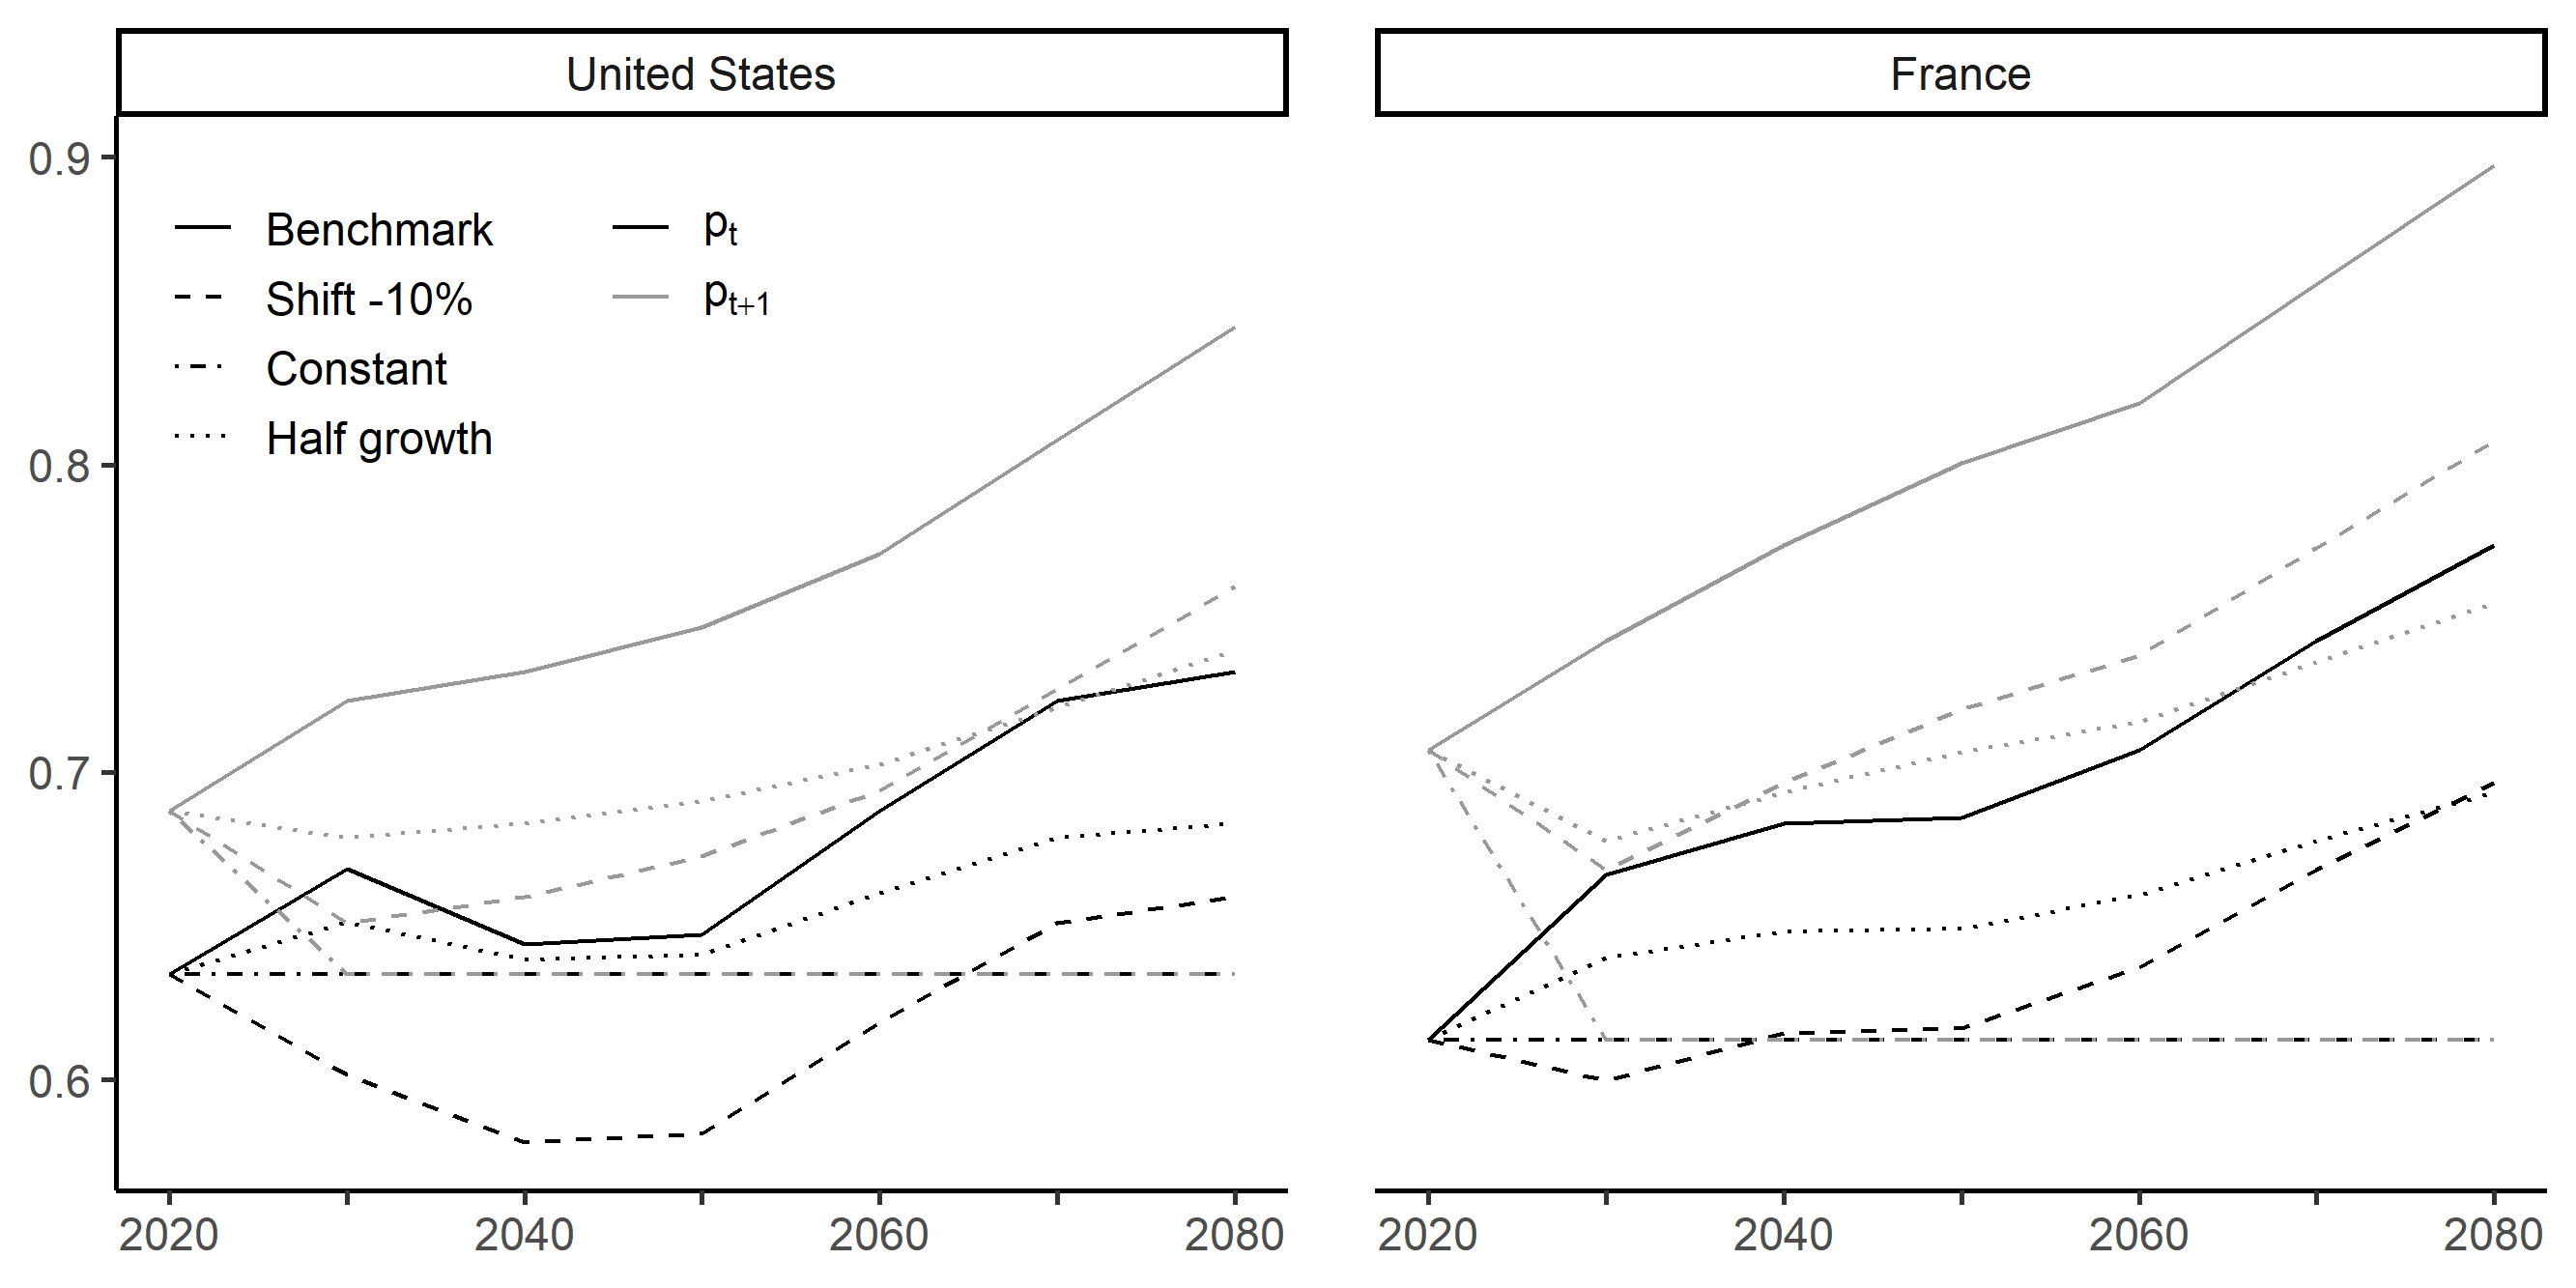
\includegraphics[width=1\linewidth]{../result/retirement/retage_p.png}
	%		\vspace{.5ex}
	%		\hrule
	%		\vspace{-4ex}
	%		\justify\singlespacing\footnotesize 
\end{figure}
The dashed curves correspond to the first scenario mentioned above where the survival rate is shocked by -10\% in 2030 and keeps its growth rate thereafter. The dash-dotted and dotted curves are two special cases of the second scenario. The dashed-dotted curves refers to the case where $\zeta = 0$, so the survival rate remains constant after 2030. It means that variations in retirement age are fully proportional to those in life expectancy. While the dotted curves coincide to the case where $\zeta = .5$. Thus, the survival rate $p_t$ grows at half of the speed of the benchmark simulation.

Figure \ref{fig:retage_ls} displays model predictions of the labor share according to the scenario.
\begin{figure}[tb]
	\centering
	\caption{Model predictions of the labor share with changing retirement age specifications} \label{fig:retage_ls}
	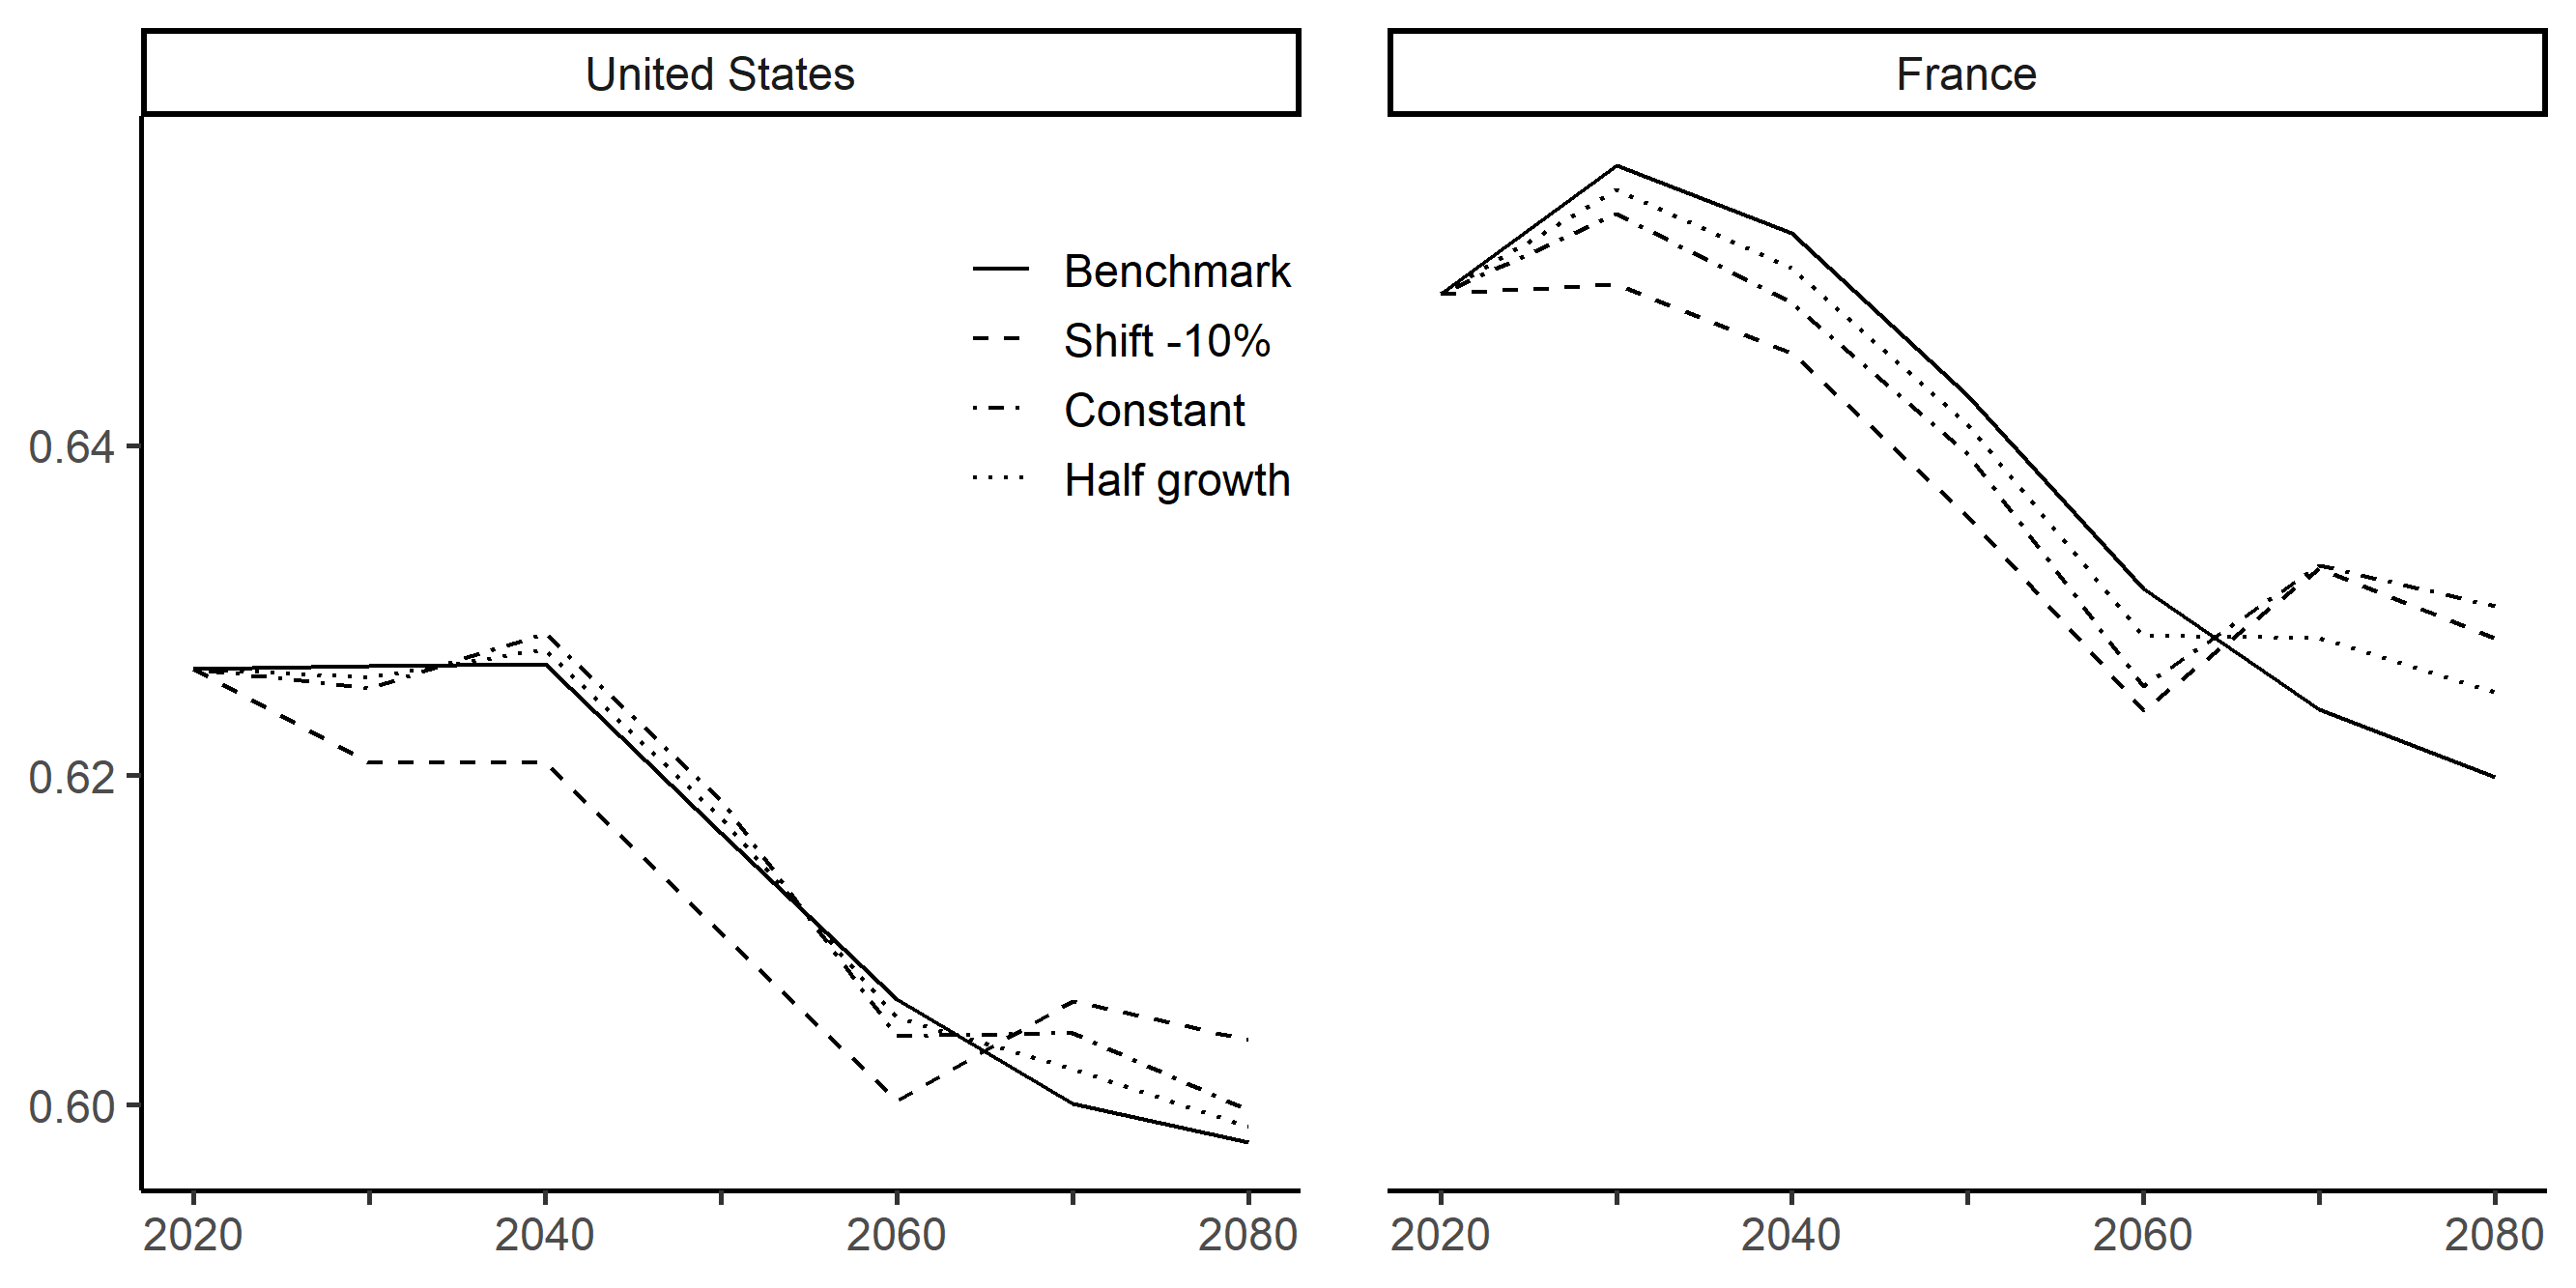
\includegraphics[width=1\linewidth]{../result/retirement/retage_ls.png}
%		\vspace{.5ex}
%		\hrule
%		\vspace{-4ex}
%		\justify\singlespacing\footnotesize The solid black curve corresponds to the labor share from the benchmark prediction. Dashed curves correspond to different changes in retirement age. \textit{Shift -10\%} corresponds
\end{figure}
The raise of the age of retirement in France leads to a decline of the labor share with respect to the benchmark simulation in a first phase. In a second phase, the very long-run, the labor share is relatively greater than in the benchmark case. This result holds regardless of the scenario. In the United-States, the impact on the labor share depends on the scenario. As in France, the -10\% shift scenario generates a sharper decline of the labor share before to exceed the benchmark simulation's one in the very long-run. However, both scenarii of diminished growth of the survival rate have roughly the same pattern of the benchmark labor share. But there are still above the labor share in the very long-run. Therefore, changing the retirement age may have different impact on the labor share according to the country.

% Mechanisms
The underlying mechanisms are related to those detailed in section \ref{sec:quantitative_analysis}. However, there is a particularity to this change of the retirement age. The capital stock does not immediately adjust in the model. Because it has been determined by the savings of the previous period of each sequence, where the expected survival rate $p_{t+1}$ was much greater than the after-reform one $p^\prime_{t+1}$. This specificity cancels part of the direct cohort effect. This relatively high amount of available capital stock plays in favor of the firm within the wage bargaining. Because the firm is all the more able to substitute labor with capital. On the indirect cohort effect's side, the agents remain young longer due to the increase of the retirement age. This is translated in terms of the model with a decrease of the number of old households and an increase of the number of young households. Thus, the youth has more political weight than in the benchmark case. With this political strength, they raise their outside option through pro-young public policies which allows them to bargain greater wages. As a response, the firm shift away from labor and hire relatively less workers than in the benchmark case. As mentioned above, the relatively high amount of available capital stock due to the \textit{stickiness} enables the firm to substitute all the more.

